\documentclass[10pt, a4paper]{article}
\usepackage{fullpage}
\usepackage{graphicx}
\usepackage{subcaption}

\DeclareGraphicsExtensions{.jpg}

\setlength{\parskip}{0.3cm}
\setlength{\parindent}{0cm}

\begin{document}
\title{Planning, Estimating and Tracking
\\ 3D Heap Visualisation}
\author{Briony Goldsack, Aviv Beeri, Ying Jiang, Oliver Myerscough, 
\\ Anna Thomas, Eleanor Vincent}
\maketitle

\section{Introduction} 
An object-oriented software application creates complex structures on the heap during its lifetime. Debugging object-oriented software often involves thinking about how the heap evolves as the program runs. The aim of our group project is to design a tool which supports visualisation of the heap of a running Java program as a 3D scene, which can then be navigated by the user through first person perspective. 

This report aims to present the planning, estimations and project management techniques that we have chosen to implement in the initial development stages of our 3D Heap Visualisation Tool. The report will discuss the requirements that we have successfully formalised using ‘use case analysis’, the current work plan going forward, detailing the division of labour, and the tools we have chosen to apply to keep track of tasks and issues. This report also includes feedback on our initial plan from the group supervisor, Alastair Donaldson. 

\section{Project Requirements}

\subsection{Use Case Analysis}

We chose to implement use case analysis to structure our requirements process so as to enable us to first consider the requirements of our heap visualisation tool at a higher level using user stories and then develop the specifications from these, using actors and use cases. Having received feedback on our user stories from our supervisor, these then morphed into our final requirements specific use cases. Our first step in creating user stories was to envision our end users (actors within each use case). We identified three initial applications of our heap visualisation tool: education, gaming, debugging, which gave us an insight into our ‘actors’:

\begin{itemize}

  \item Teacher/Lecturer
  \item Beginner Programmer
  \item Experienced Programmer 
  \item A Typical Gamer 

\end{itemize}

We decided to combine the agile development user story strategy with methods introduced in the HCD course in the form of personas to allow us to imagine in more detail scenarios in which our heap visualisation tool could be used.

\textbf{James Dawkins} 
\\ Lecturer at Imperial College, London. James teaches Java programming to first-year students, some of whom have never programmed before or used an object-oriented language. James likes to deliver interactive lectures, but also must create worksheets for tutorials and feels that students learn best by ‘doing’. 

\begin{figure}[h]
        \centering
        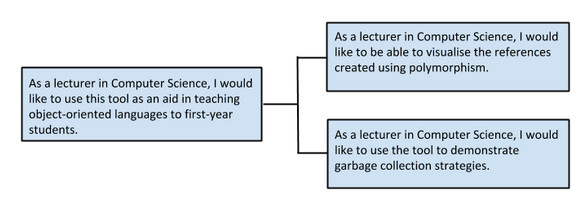
\includegraphics[width=\textwidth]{images/user1.jpg}
\end{figure}

\textbf{Randall Jones}
\\ Programmer at GenericSoftwareCompany™. Randall frequently works on developing large computer systems in object-oriented languages. Randall primarily programs using the Linux operating system.

\begin{figure}[h]
        \centering
        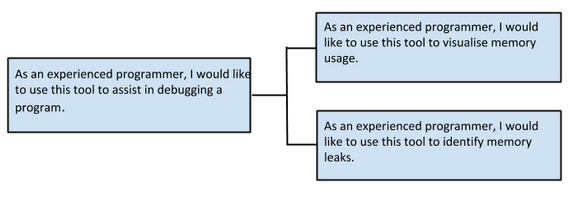
\includegraphics[width=\textwidth]{images/user2.jpg}
\end{figure} 

\textbf{Bethan Fielding}
\\ First-year Computing Student at Imperial College London. Bethan has previously done some programming with HTML and CSS to create websites, however has never used an object-oriented language like Java, an IDE or compiler.

User Story: “As a beginner to programming, encountering an object-oriented language for the first time, I would like to use this tool in order to understand the heap as well as features of object-oriented programming.”

\textbf{John Barden}
\\ Post-graduate in Biology at Imperial College, with a love of gaming. While writing up his thesis, John enjoys playing quick games to break up the day. He has played a number of games which use the surrounding environment, e.g. the music he is listening to, to generate maps for games such as racing or first-person-shooter, and John often picks games to play based on their visual aesthetics.

User Story: “As a gamer, I would like to use this tool to play quick games that don’t risk taking up hours and hour of my time but remain interesting throughout each run.”

Our current use case actors could be extended to include systems that play a role within our heap visualisation tool. For example, if we were to create a plugin for Eclipse or IntelliJ, these systems would be considered actors within certain use cases as other actors interact with them. The Experienced Programmer, Beginner and Gamer extend a General User role as both may want to navigate the heap, visualise object references, read object information and mark objects. However, there are also specific use cases.
\\

\noindent Use cases:
\begin{itemize}

  \item Navigate heap in real-time
  \item Visualise object references
  \item Read object information
  \item Mark/write on objects 
  \item Visualise memory usage

\end{itemize}

\noindent Specific use cases:
\begin{itemize}

  \item Learn garbage collection strategies
  \item Identify memory leaks
  \item Game Play
  \item Visual Appreciation

\end{itemize}
In developing our use case analysis to create our requirements, it was also important to consider alternate flows as well as ideal scenarios (the basic flow). Alternate flows that could: be encoutered within the heap visualisation tool include:
Encountering an exception while debugging
Incorrect student solution to programming task

While developing our tool we plan to keep our use cases agile by adapting them as requirements are refined. Having carried out our use case analysis, we identified a set of initial base requirements, which we feel are essential to the project, as well as a set of requirements which we would like to implement.
\\

\noindent Base Requirements
\begin{itemize}

  \item Dynamic extraction of heap information
  \item 3D interactive space
  \item Intuitive heap navigation
  \item Visualisation of objects on the heap and references between them
  \item Ability to obtain object information (e.g. address, type, etc.) 
  \item Ability to mark objects or leave notes within the 3D space
  \item Easy to install

\end{itemize}

\noindent Extended Requirements
\begin{itemize}

  \item Cross-platform tool
  \item Ability for a lecturer to set an assignment
  \item Post-processing heap analysis to aid debugging
  \item Game features

\end{itemize}

\section{Project Plan}

This section will detail our plan going forward for the development of the heap visualisation tool, including our preliminary estimations of how long we expect these features to take. We will describe how we have come up with this current plan and how we plan to manage the various tasks. 

\subsection{Planning Poker}

Throughout our project we will be doing weekly sprints, we have chosen weekly sprints due to our time constraint of 9 weeks. This allows us sufficient time to complete features within each sprint and still gives us many milestones to adjust our plan depending on how much work had been completed that week. Planning poker is a consensus-based technique used to estimate the effort that will be required to complete each feature we are planning on implementing. Before playing the group must have a list of features that they want to be implemented over the given time frame (in this case one week), this feature list should be based on user stories capturing the ‘what’ and ‘why’ of each feature. Planning poker uses multiple sets of cards numbered 0, 0.5, 1, 2, 3, 5, 8, 13, 20, 40, 100 where 100 represents 100\% of the time and effort. Each player has a deck of cards and plays their card based on how much time and effort they believe the feature will require, once all players have played their cards they are all revealed simultaneously. We played planning poker at the start of our sprint this week using the whole 9 weeks as our time frame to decide which features we should be able to implement by the end of the project, the results have been plotted in the gantt chart below. At the beginning of each sprint from now on we will reevaluate our plan and use the ideas of planning poker to agree on what we can achieve in the next week.

Hiding the cards until everyone has played is extremely beneficial in making estimates as it minimises anchoring (early comments by team members that "anchor" a task time by expressing it aloud) which can occur if team estimates are made based on discussion alone. This also exposes the potentially influential team members as being isolated in their opinion then allows them to argue their case against the majority, this way the less influential team members can have faith in their original estimates and have a more fair discussion without anchoring. Tasks estimated with planning poker tend to be less optimistic and are more accurate than the mechanical combination of individual estimates for the same tasks\textsuperscript{\cite{omgnames}}. Planning poker also helps us determine which players are on the critical path. As some players are naturally better at estimating than others so when rushing to meet a deadline critical tasks can be shifted to the people with a proven record of meeting their estimates. It also allows us to see for ourselves how good an estimator we are, this allows us to improve and make more accurate predictions in future. As our project needs to be completed in 9 weeks it’s compulsory that we are aware of which critical features are required in the end product and how long it will take to complete them, by playing planning poker we have a historical record of how long each feature has taken to complete, which features we have left and an estimate of how long we believe they will take to implement.

\begin{figure}[h]
        \centering
        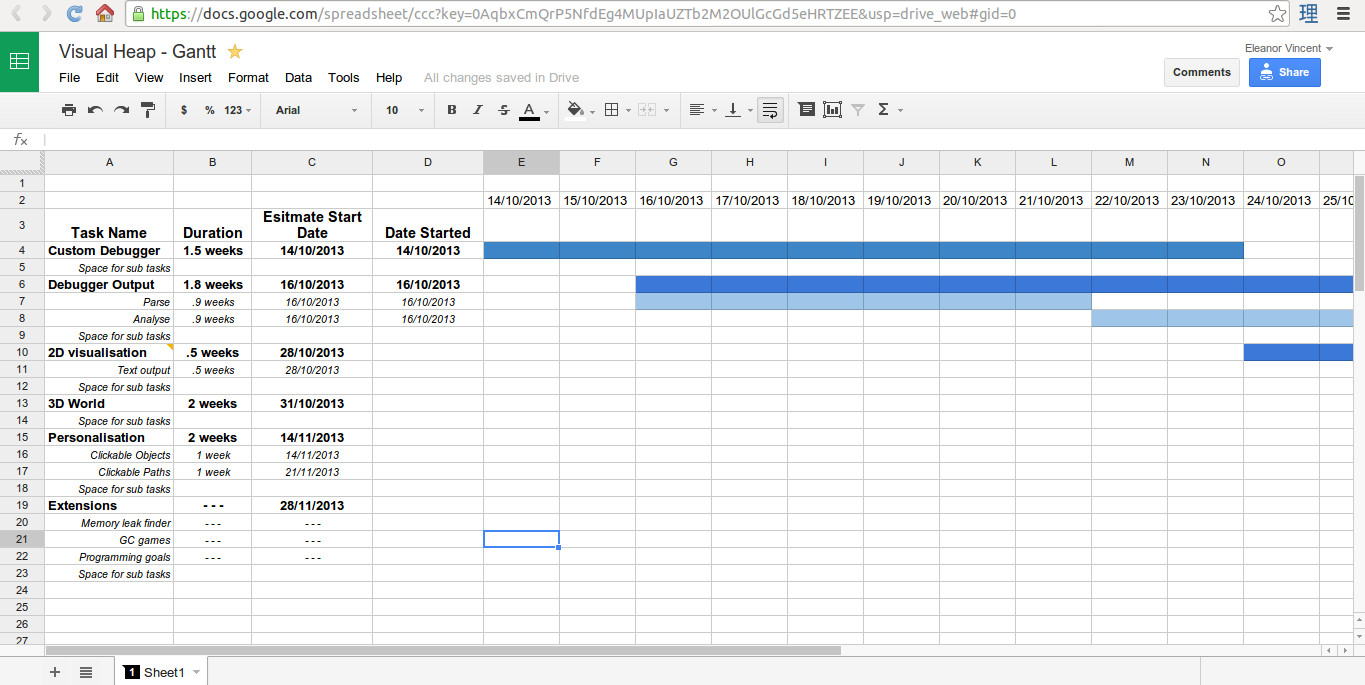
\includegraphics[width=\textwidth]{images/gantt.jpg}
        \caption{Google Drive Gantt Chart}
\end{figure}

\noindent Feature List
\begin{itemize}

  \item Custom, minimalistic debugger - 1.5 weeks
  \item Extract useful run-time heap information
  \item Parse and analyse debugger output - 1 week
  \item 2D visualisation of objects and references 
  \item 3D world (basic 3D representation of 2D map) - 1 week
  \item Interactive 3D world (clicking on objects, clicking on paths) - 1 week
  \item Personalisation (marking objects, notes on walls) - 1 week

\end{itemize}

\section{Project Management}

As a group the way we have been managing in our work has been predominantly through the project management website, trello.com. This is a useful website based on the kanban system. Each board allows you to make lists and assign cards to them; each card can then be assigned to a member of the board. It has its limitations but is useful in a situation where not all of the members can be central to one particular wall for a more low-tech approach.

To compliment this, most of our discussions have been central to various google documents that we have posted to the trello board. Most google documents have a working chat feature which is convenient when not all members are present around the same table. These represent our own version of quick 'stand-up' meetings where various members get together periodically to aid one another and take stock of their current thoughts and issues. The benefit of this being through online chat systems is that they enable a record of conversation that other members can skim through and highlight their own thoughts if required. We have also organised repeated weekly meetings; one mid-week meeting with the project supervisor to report our progress and highlight any issues that have occurred, and one end-of-week meeting amongst the team to take stock of which objectives have been reached and what should be completed by the next meeting. 

\begin{figure}[h]
        \centering
        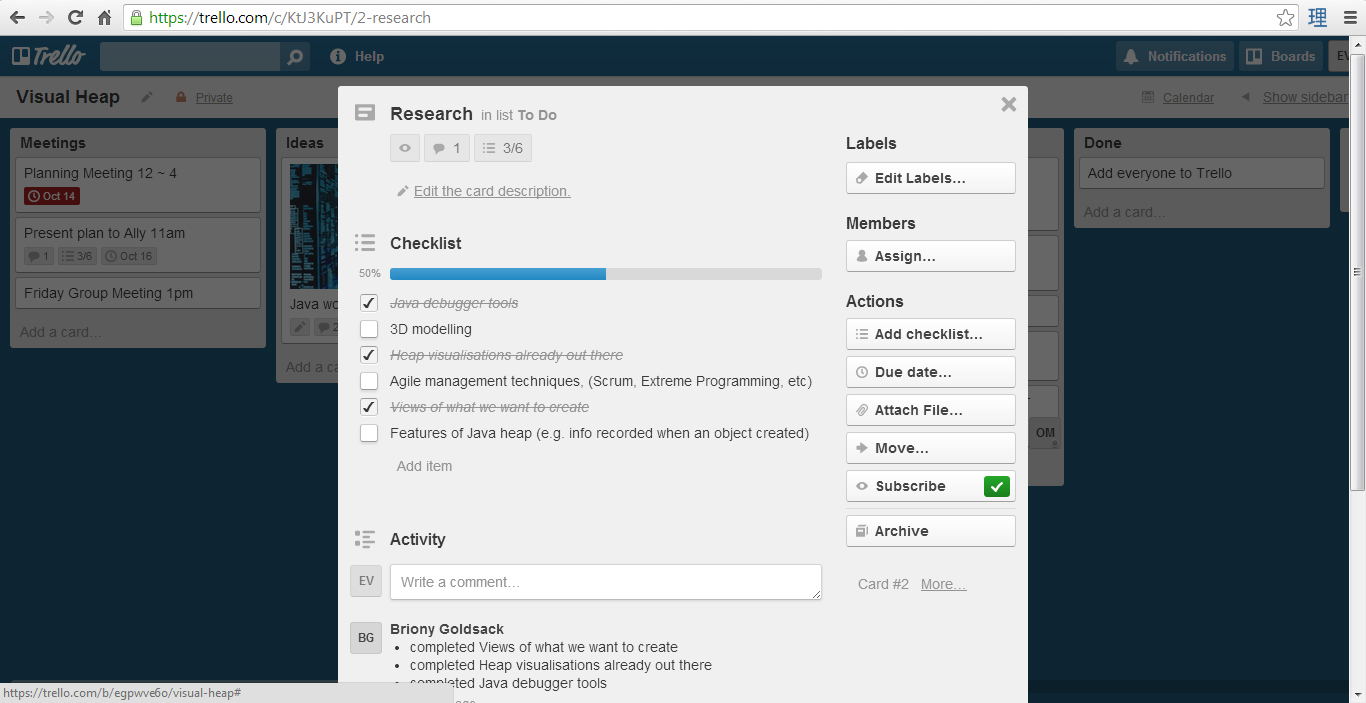
\includegraphics[width=\textwidth]{images/trello1.jpg}
        \caption{Trello Card}
\end{figure}

Reading various articles\textsuperscript{\cite{ssagile,atlasagile}} on the agile development system gave a much better understanding of the process as a whole. There are some interesting points that we had never considered, making our weekly meetings more concrete in terms of ‘stand-up’ meetings enables us to maintain our productivity throughout the project and aids in communication in a long-term sense. There are points within the system that we dislike. Sometimes it can feel counter-intuitive to spend so much time on planning documents and physical organisation and this can detract from actual product creation time, however on further consideration the boons to this effort to do seem to outweigh the potential problems that could be caused if this information were not available.

To keep track of the product itself we have opted to store and work within a private git repository. Git has an excellent array of features for keeping track of the amount of useful code provided by each member and branching options to test certain aspects without fear of corrupting the entire piece. The website github.com also hosts an issue tracker which will be convenient to use to highlight issues to one another that certain members are struggling with. This will make responses quicker and will also keep a backlog of events at the same time.
 
\section{Supervisor Discussion}

We met with our supervisor, Alastair Donaldson on 16th October to present our progress so far and our project plan. The presentation detailed our final requirements and applications acquired through case analysis, the background research we had carried out to assess the feasibility of our plan, the division of labour, a few preliminary test cases and our ideas for the interface of the tool. Alastair seemed pleased with our progress and we discussed some further applications. Alastair suggested an additional use case for those who simply want to view the heap in a different and more visually appealing way or in appreciation of the graphics. Alastair also thought that we should give more emphasis to the gaming user story as a viable application of the heap visualisation tool. Furthermore, we discussed the timescale of the project and adaptations to agile development. 

\begin{thebibliography}{9}

\bibitem{ssagile}
  Steffan Surdek,
  \emph{Agile Planning in Real Life},
  \\http://www.ibm.com/developerworks/library/l-agile-plan/

\bibitem{atlasagile}
  Atlassian,
  \emph{Do Agile Right},
  \\https://www.atlassian.com/agile/
  
\bibitem{omgnames}
  Molokken-Ostvold, K., Simula Res. Lab., Lysaker, Haugen, N.C.,
  \emph{Software Engineering Conference, ASWEC 2007},
  18th Australian,
  \\http://ieeexplore.ieee.org/xpl/articleDetails.jsp?reload=true{\&}arnumber=4159687
  
\bibitem{agilelevy}
  Darren Levy,
  \emph{Use Case Examples - Effective Samples and Tips},
  \\http://www.gatherspace.com/static/use{\_}case{\_}example.html

\end{thebibliography}

\end{document}